\emph{Cancer} is an umbrella term for a group of diseases caused by abnormal cell growth in different parts of the body. The accumulation of extra cells usually forms a mass of tissue called a \emph{tumor}. Tumors can be benign or malignant: \emph{benign tumors} are noncancerous, lack the ability to invade surrounding tissue and will not regrow if removed from the body;  malignant or \emph{cancerous tumors} are harmful, can invade nearby organs and tissues (\emph{invasive cancer}), can spread to other parts of the body (\emph{metastasis}) and will sometimes regrow when removed~\cite{WYNTKABreastCancer2012}.

\emph{Breast cancer} forms in tissues of the breast. The two most common types of breast cancer are \emph{ductal carcinoma} and \emph{lobular carcinoma}, which start in the breast ducts and lobules, respectively (see Fig.~\ref{fig:BreastAnatomy}). Breast cancer \emph{incidence rate}, the number of new cases in a specified population during a year, is the highest of any cancer among American women. Its \emph{mortality rate}, the number of deaths during a year, is also one of the highest of any cancer~\cite{Howlader2014}.

\begin{figure}[h]
	\centering
	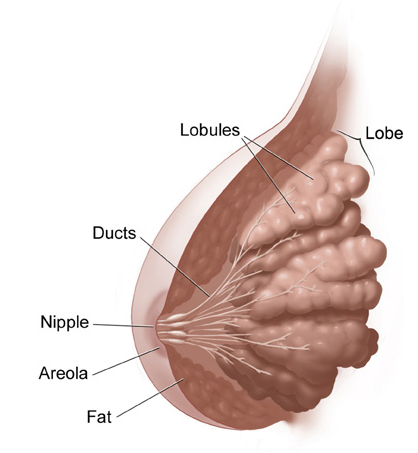
\includegraphics[width = 0.35\textwidth]{plots/breastAnatomy.png}
	\caption[Anatomy of the female breast]{Anatomy of the female breast. Image courtesy of NCI.}
	\label{fig:BreastAnatomy}
\end{figure}

The \emph{cancer stage} depends on the size of the tumor and whether the cancer cells have spread to neighboring tissue or other parts of the body. It is expressed as a Roman numeral ranging from 0 through IV; stage I cancer is considered \emph{early-stage breast cancer} and stage IV cancer is considered \emph{advanced}. Stage 0 describes non-invasive breast cancers, also known as \emph{carcinoma in situ}. Stage I, II and III describe invasive breast cancer, i.e., cancer has invaded normal, surrounding breast tissue. Stage IV is used to describe metastatic cancer, i.e., it has spread beyond nearby tissue to other organs of the body.

%\subsection{Mammograms}
\subsubsection{Mammograms}
A \emph{mammogram} is an x-ray image of the breast. Radiologists use \emph{screening mammograms} (normally composed of two mammograms of each breast) to check for breast cancer signs on women who lack symptoms of the disease. If an abnormality is found, a \emph{diagnostic mammogram} is ordered, these are detailed x-ray pictures of the suspicious region~\cite{Mammograms2014}. A standard mammogram is shown in Fig.~\ref{fig:normalMammogram}.

\begin{figure}[h]
	\centering
	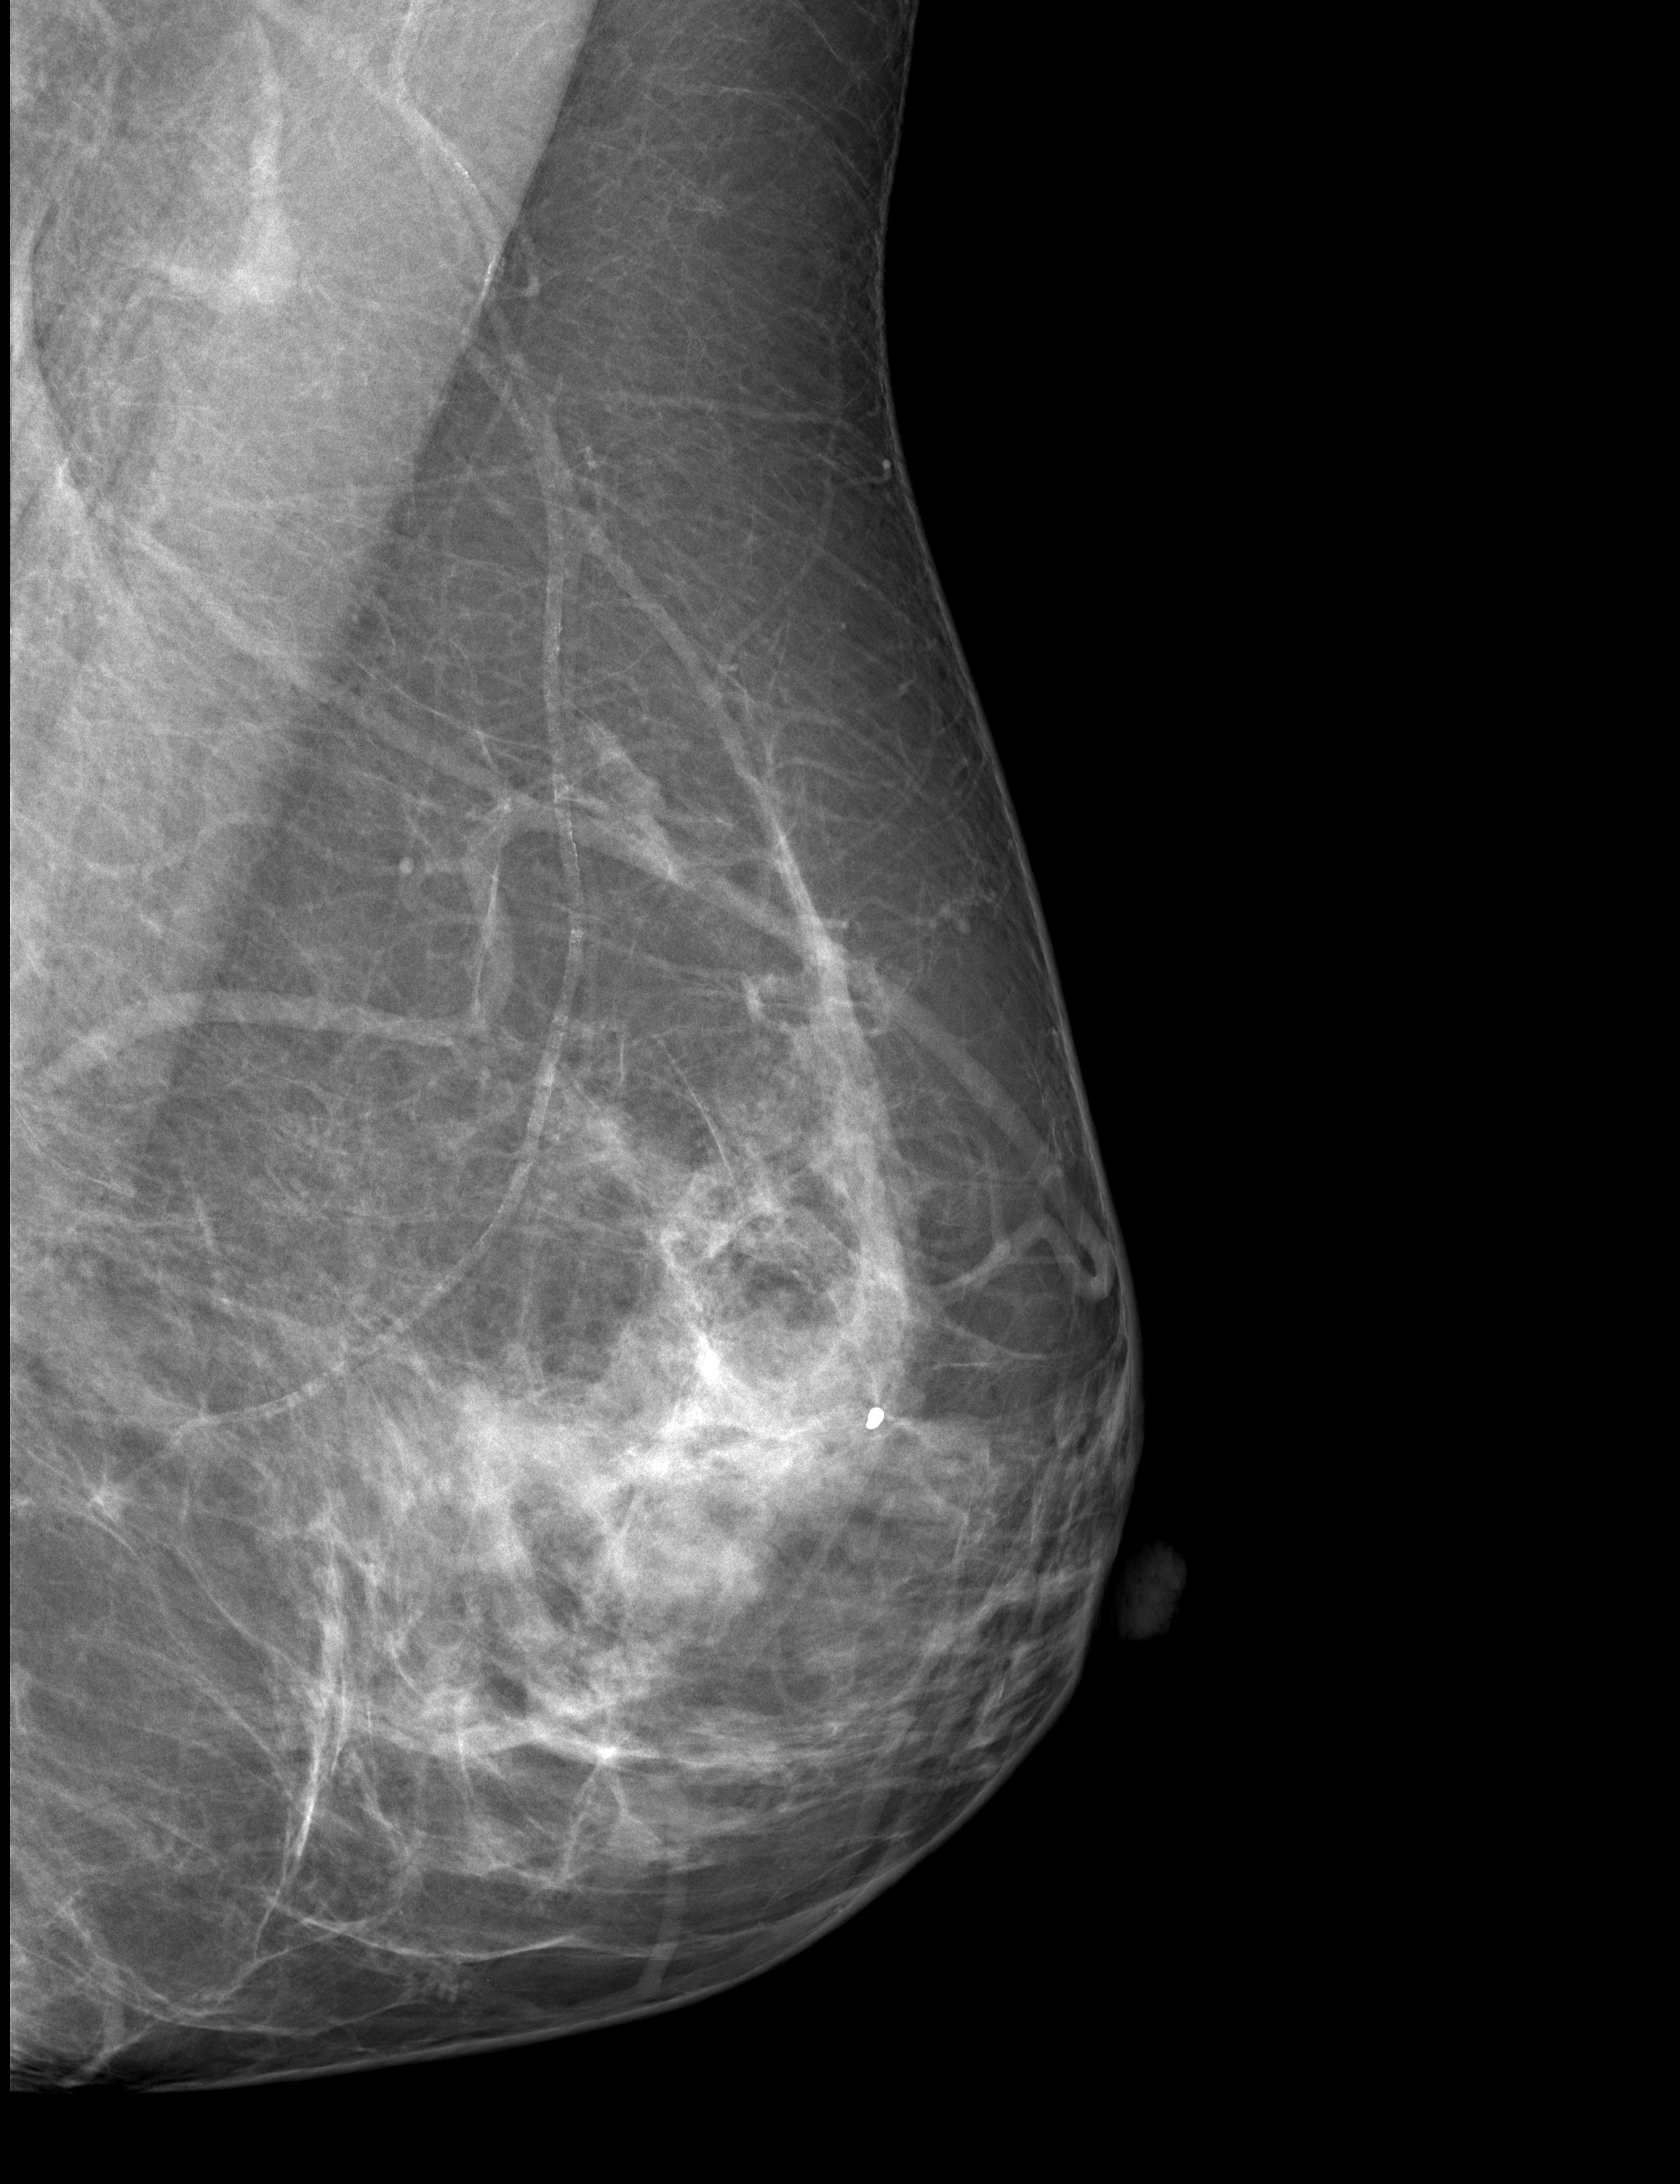
\includegraphics[width = 0.26\textwidth]{plots/normalMammogram.jpg}
	\caption[A digital mammogram]{A standard mammogram.}
	\label{fig:normalMammogram}
\end{figure}

Having a screening mammogram in a regular basis is the most effective method for detecting breast cancer early; around 85\% of breast cancers can be detected in a screening mammogram~\cite{PerformanceMammography2013}. Nevertheless, screening mammograms have many limitations: a high false positive rate, overtreatment in Stage 0 cancer, false negative results for women with high breast density, radiation exposure and physical and psychological discomfort~\cite{Mammograms2014}.

Radiologists look primarily for microcalcifications and breast masses. \emph{Microcalcifications} are tiny deposits of calcium in the breast tissue that can be a sign of early breast cancer if found in clusters with irregular layout and shapes. \emph{Breast masses} or breast lumps are a variety of things: fluid-filled cysts, fatty tissues, fibric tissues, noncancerous or cancerous tumors, among others. A mass can be a sign of breast cancer if it has an irregular shape and poorly defined margins. See Fig.~\ref{fig:breastCancerSigns} for an example of signs of breast cancer. Radiologists will also consider the breast density of the patient when reading a mammogram given that high breast density is linked to a higher risk of breast cancer~\cite{MammogramsACS2014}.

\begin{figure}[h]
	\centering
	\begin{subfigure}{0.25\textwidth}
                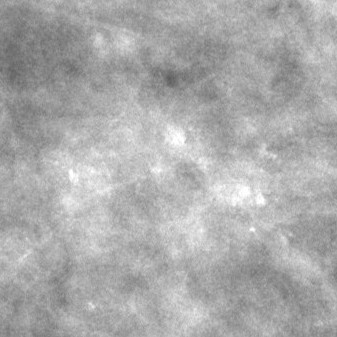
\includegraphics[width=\textwidth]{plots/breastMicrocalcification.jpg}
        \end{subfigure}
	~
	\begin{subfigure}{0.25\textwidth}
                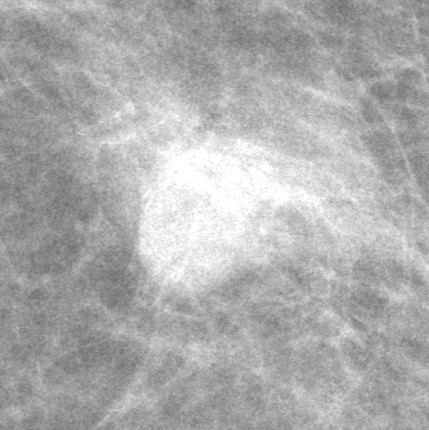
\includegraphics[width=\textwidth]{plots/breastMass.jpg}
        \end{subfigure}
	\caption[Signs of possible breast cancer]{Signs of possible breast cancer in a mammogram. Left: A cluster of microcalcifications in an irregular layout. Right: A poorly defined breast mass.}
	\label{fig:breastCancerSigns}
\end{figure}

Conventional mammography uses film to record x-ray images of the breast. \emph{Digital mammography}, on the other hand, uses digital receptors to convert the x-rays into electrical signals and stores the image electronically. Digital mammograms offer a clearer picture of the breast and can be digitally manipulated and shared between health care providers.
% However, researchers still debate whether [[its|their] use over| they] [surpass| improve on|outperform|[offers|have] an advantage over|are more effective than|benefit] film mammograms [in|for] [identifying breast cancer|breast cancer detection].
However, researchers still debate whether they offer an advantage over film mammograms~\cite{Kerlikowske2011, Pisano2008, Skaane2007}. Digital mammography is steadily becoming the standard for breast cancer screening. Fig.~\ref{fig:normalMammogram} is, in fact, a digital mammogram.

\emph{Digital tomosynthesis}, also called three-dimensional mammography, is a new technology that produces 3-dimensional x-ray images of the breast and is expected to improve the efficacy of regular 2-d mammograms. Studies comparing the two techniques have not yet been published~\cite{Mammograms2014}.

%We use digital mammograms [to train our system  and produce |detect masses and microcalcifications] and produce a valid image segmentation.
We use digital mammograms to detect breast masses and produce a valid image segmentation.

We wrote this section using information from the National Cancer Institute. We recommend to visit its website (\url{www.cancer.gov}) for further details.
